\section{Machine Translation}
\subsection{Difficulties}
\textbf{Machine translation} concerns the use of computers to automate translation from a \emph{source language} to a \emph{target language}.
This task is difficult because of
\begin{itemize}
	\item \textbf{Structural divergences}.
	\begin{itemize}
		\item \emph{Morphologically}.
		Some languages are \emph{isolating} (one morpheme per word) whereas others are \emph{polysynthetic} (multiple morphemes per word).
		\item \emph{Syntactically}.
		Languages differ in \emph{word order}.
		\item \emph{Argument structure} and linking with predicates.
		\emph{Verb-framed} languages mark the direction of motion on the verb, whereas \emph{satellite-framed} languages mark the direction on the satellite.
		\item \emph{Pronoun dropping}.
		\item \emph{Specific divergences}, e.g. order of noun and adjective.
	\end{itemize}
	\item \textbf{Lexical divergences}.
	\begin{itemize}
		\item \emph{Homonymous} words need to be disambiguated.
		\item \emph{Polysemous} words (multiple meanings) may not have the same polysemy in both languages.
		\item \emph{Grammatical lexical divergences}.
		Some languages mark gender on adjectives, others on pronouns, etc.
		\item \emph{Lexical gaps}.
		Not all words have an equivalent in both languages.
	\end{itemize}
\end{itemize}

On top of this, several translation tasks exist:
\begin{itemize}
	\item \textbf{Rough translation} (e.g. document categorization, shallow information retrieval, etc.).
	\item \textbf{Draft translation}, with \emph{human post-editing}.
	\item \textbf{Fully automatic translation}.
	For some specific \emph{sublanguage} domains with \emph{limited vocabulary}, \emph{few basic phrase types} and \emph{rare ambiguities}, this is a solved problem, but in general it is an open problem (quantum leap thanks to deep learning).
\end{itemize}

\subsection{Classical MT Approaches}
There are various possible \emph{levels of transfer}, shown in Figure~\ref{fig:levels_of_transfer}.
\begin{figure}[!hbtp]
	\centering
	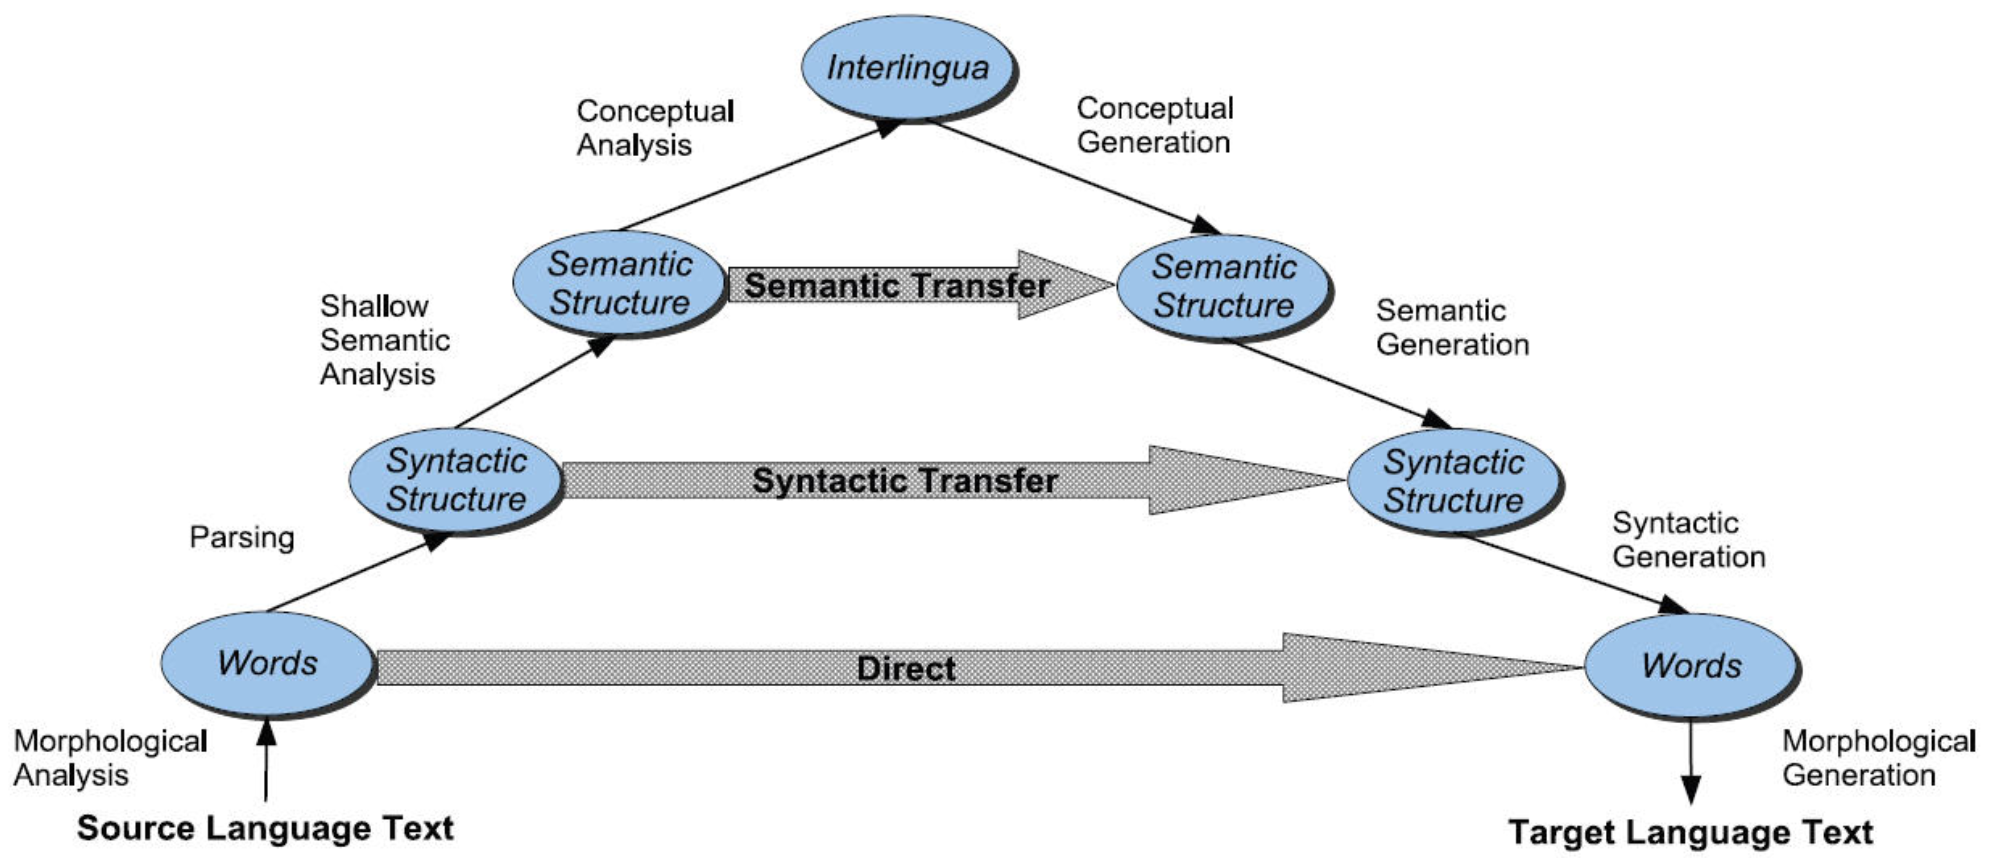
\includegraphics[width=0.8\textwidth]{img/levels_of_transfer}
	\caption{Levels of transfer}
	\label{fig:levels_of_transfer}
\end{figure}

\subsubsection{Direct Transfer}
\textbf{Direct transfer} is done \emph{word-by-word} through the \emph{source language text}, by \emph{incrementally transforming} the source language text into a target language text.
This uses a \emph{bilingual dictionary} for lexical transfer.

However, it has the following limitations:
\begin{itemize}
	\item it uses many complex transformation rules; and
	\item there is no parsing component, hence it cannot handle \emph{long distance reordering}.
\end{itemize}

\subsubsection{Syntactic and Semantic Transfers}
The \textbf{syntactic transfer} approach uses the following steps:
\begin{enumerate}
	\item \emph{parse};
	\item \emph{transfer} the syntactic structure;
	\item \emph{generate} the target text.
\end{enumerate}

This has the following limitations:
\begin{itemize}
	\item Some translations require \emph{complex syntactic transformations}.
	\item \emph{Lexical transfer} is required with a \emph{bilingual dictionary}, but this does not take care of \emph{ambiguous words}.
	\item Additional \emph{semantic analysis} is required but it is \emph{even more complex} to define reliable semantic transformations.
\end{itemize}

\subsubsection{Interlingua}
The previous approaches need to be implemented with \emph{distinct rules} for \emph{each language pair}.
For this reason, the idea of \textbf{Interlingua} was proposed.
In this idea, translation is treated as a process of \emph{extracting the full meaning of the source} and \emph{expressing it in the target} language.

This has the following limitations:
\begin{itemize}
	\item Deep conceptual analysis is even harder than shallow semantic analysis.
	\item The generation steps are far from trivial.
	\item Some concepts do not exist in both languages (lexical gaps).
\end{itemize}

\subsection{Statistical Machine Translation}
The \textbf{statistical approach} is based on the following simple idea: \emph{focus} on the \emph{result}, not the process.
This allows us to define that the \emph{best} translation \(\hat{T}\) is the one that maximizes the \emph{faithfulness} but also the \emph{fluency} of the translation:
\[
\hat{T} = \argmax_{T} \big(\mathrm{faithfulness}(T, S) \, \mathrm{fluency}(T)\big).
\]

More formally, we have the following problem: \emph{given} a \emph{source} language sentence \(S = s_1, \dots, s_M\), \emph{find} the \emph{target} language sentence \(T = t_1, \dots, t_N\) \emph{maximizing} \(\Pr(T \mid S)\):
\[
\hat{T} = \argmax_{T} \Pr(T \mid S) = \argmax_T = \underbrace{\Pr(S \mid T)}_{\substack{\textnormal{translation} \\ \textnormal{model}}} \underbrace{\Pr(T)}_{\substack{\textnormal{language} \\ \textnormal{model}}}.
\]

This means that statistical MT requires
\begin{itemize}
	\item a \emph{target language model} to compute \(\Pr(T)\) (\(N\)-grams);
	\item an (inverse) \emph{translation model} to compute \(\Pr(S \mid T)\);
	\item a \emph{decoder} to compute \(\hat{T} = \argmax_T \Pr(S \mid T) \Pr(T)\).
\end{itemize}

Our \textbf{translation model} is built on the principle of \emph{phrase-based alignments}, where \emph{phrases} (as well as single words) are used as the \emph{units of translation}.
Since \emph{each phrase} has exactly \emph{one translation}, \emph{alignments are permutations}.
The model includes \emph{translation probabilities} of phrases and \emph{distortion probabilities} to model the permutations.

The translation model is built using 
\begin{itemize}
	\item \emph{phrase translation probabilities} \(\Pr(\bar{s}_i \mid \bar{t}_i)\), and
	\item \emph{distortion probabilities} \(d(a_i, b_{i-1}) = \alpha^{\abs{a_i - b_{i-1} - 1}}\), to penalize ``strong'' permutations, where
	\begin{itemize}
		\item \(a_i\) is the start word position of the source phrase generated by the target phrase \(\hat{t}_i\);
		\item \(b_{i-1}\) is the end word position of the source phrase generated by the target phrase \(\hat{t}_{i-1}\), with \(b_0 = 0\);
		\item \(\alpha\) is a small positive constant.
	\end{itemize}
\end{itemize}
It is given by
\[
\Pr(S \mid T) = \prod_{i = 1}^{\ell} \Pr(\hat{s}_i \mid \hat{t}_i) d(a_i, b_{i-1}).
\]

The parameters of this model are \(\Pr(\hat{s} \mid \hat{t})\) for a large collection of parameters and \(\alpha\), which are learnt in what is essentially a \emph{large bilingual probabilistic dictionary} of \emph{phrases} which can be estimated from a large corpus of \emph{aligned phrases} and their respective \emph{counts} (with smoothing):
\[
\Prhat(\bar{s} \mid \bar{t}) = \frac{C(\bar{s}, \bar{t})}{\sum_{\bar{s}'} C(\bar{s}', \bar{t})}.
\]

However, aligned phrases are \emph{rarely available} in parallel corpora.
In practice, \emph{word alignments} are often used as \emph{seeds} for phrase alignment.
This strategy works as follows:
\begin{enumerate}
	\item \emph{Symmetrize}: produce word alignments \(S \to T\) and \(T \to S\).
	\item \emph{Intersect} both alignments.
	\item Build a \emph{classifier} to select additional connections from the \emph{union} of both alignments.
	\item Extract \emph{consistent phrases}.
\end{enumerate}

The \emph{decoding} step is concerned with finding
\[
\hat{T} = \argmax_{T} \Pr(S \mid T) \Pr(T) = \argmin_{T} \mathrm{cost}(S, T).
\]
Typically, \emph{best-first search} algorithms (such as A\textsuperscript{*}) are used to find the minimal cost solution.
The \emph{cost} combines
\begin{itemize}
	\item the \emph{current cost} of \emph{currently translated phrases} (\(S_{1, \dots, j}, T_{1, \dots, j}\)):
	\[
	\mathrm{cost}(S_{1, \dots, j}, T_{1, \dots, j}) = -\log \left(\prod_{i = 1}^j \Pr(\bar{s}_i \mid \bar{t}_i) d(a_i, b_{i-1}) \Pr(T_{1, \dots, j})\right),
	\]
	\item the \emph{future cost} to translate the remaining words, which is estimated by \emph{ignoring} distortion costs.
\end{itemize}
This algorithm is referred to as \textbf{multi-stack decoding}, but uses \emph{priority queues} in practice.
The ``stack'' \(s_m\) stores all current hyptheses covering the same number \(m\) of source phrases.
An alternative is the \emph{beam-search decoder}, which develops the top-\(K\) hypotheses in a BFS (same fraction of the source sentence), and prunes the others.

\subsection{MT Evaluation}
A sentence could be translated in different ways, according to different criteria:
\begin{itemize}
	\item \textbf{Human raters}.
	\begin{itemize}
		\item \emph{fluency}: clarity, naturalness or style;
		\item \emph{faithfulness}: adequacy (same information as source);
		\item \emph{informativeness}: enough information to complete a task;
		\item \emph{edit cost}: minimize required human editing.
	\end{itemize}
	\item \textbf{Automatic evaluation}.
	Heuristics are used to \emph{assess} translation systems \emph{automatically} w.r.t. reference translations provided by humans.
	Not necessarily equivalent, but \emph{correlated with human judgment}.
\end{itemize}

\paragraph{\(N\)-gram precision}
The \textbf{\(N\)-gram precision} metric simply counts how many \(N\)-grams (for various \(N\)) are in \emph{common} between the \emph{candidate translation} and some \emph{reference translations}.
However, this metric favors a candidate repeating a few words present in the references multiple times.
A \emph{recall measure} is not relevant, since not all reference \(N\)-grams have to appear in the candidate.

\paragraph{Modified \(N\)-gram precision}
To solve the problem above, the \textbf{modified \(N\)-gram precision} metric adds the rule that a specific candidate \(N\)-gram is counted at most the number of times it appears in a single reference, which we call \emph{clipped \(N\)-gram counts}.

\paragraph{BLEU metric}
To obtain the \textbf{BLEU metric} (BiLingual Evaluation Understudy), we add a \emph{brevity penalty}, which penalizes exceedingly short candidates.
The BLEU metric is computed over a \emph{whole test corpus} with one candidate per translated segment, and several references.
The \emph{modified \(N\)-gram precision} \(p_n\) for \(N\)-grams \(g\) of order \(n = 1, 2, \dots, N'\) is given by
\[
p_n = \frac{\sum_{C \in \textnormal{candidates}} \sum_{g \in C} C_\textnormal{clipped}(g)}{\sum_{C \in \textnormal{candidates}} \sum_{g \in C} C(g)}.
\]
The brevity penalty is defined as
\[
\textnormal{BP} = \left\{\begin{array}{l@{\quad}l}
1, & \textnormal{if} \quad \abs{C} > \abs{R} \\
e^{1 - \frac{\abs{R}}{\abs{C}}}, & \textnormal{if} \quad \abs{C} \leq \abs{R},
\end{array}\right.
\]
where
\begin{itemize}
	\item \(\abs{C}\) is the sum of the lengths of the candidate translations; and
	\item \(\abs{R}\) is the sum of the lengths of the best-matching reference for each candidate.
\end{itemize}
The full BLEU metric is then expressed as
\[
\textnormal{BLEU} = \textnormal{BP} \cdot \exp\left(\frac{1}{N'} \sum_{n = 1}^{N'} \log p_n\right).
\]
Note that the precision term corresponds to the geometric average of the modified \(N\)-gram precisions.